% Created by tikzDevice version 0.12.3.1 on 2022-09-02 16:29:21
% !TEX encoding = UTF-8 Unicode
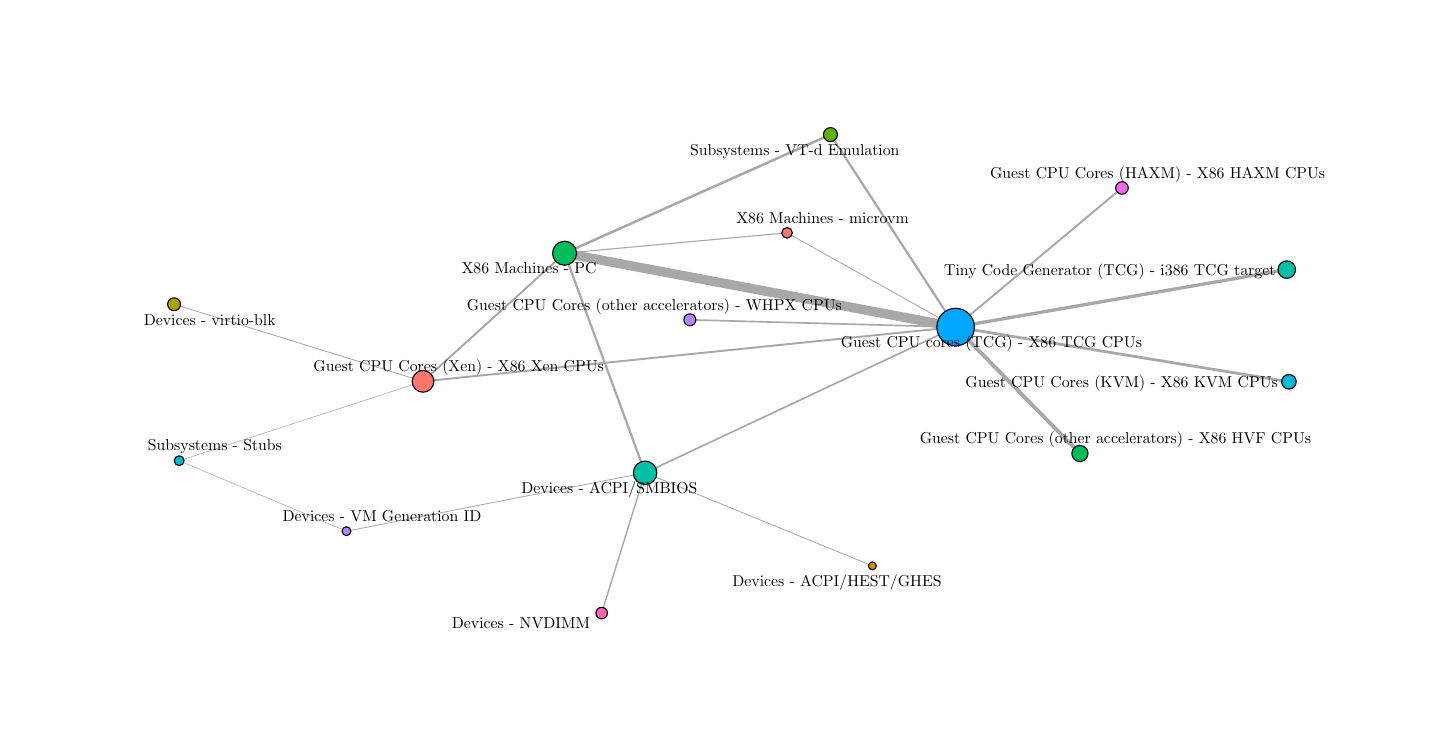
\begin{tikzpicture}[x=1pt,y=1pt]
\definecolor{fillColor}{RGB}{255,255,255}
\path[use as bounding box,fill=fillColor,fill opacity=0.00] (0,0) rectangle (505.89,252.94);
\begin{scope}
\path[clip] (  0.00,  0.00) rectangle (505.89,252.94);
\definecolor{fillColor}{RGB}{255,255,255}

\path[fill=fillColor] (  0.00,  0.00) rectangle (505.89,252.94);
\end{scope}
\begin{scope}
\path[clip] ( 32.75, 32.75) rectangle (475.89,222.94);
\definecolor{drawColor}{gray}{0.66}

\path[draw=drawColor,line width= 0.3pt,line join=round] (305.23, 58.46) -- (223.11, 92.09);

\path[draw=drawColor,line width= 0.5pt,line join=round] (223.11, 92.09) -- (207.41, 41.40);

\path[draw=drawColor,line width= 0.3pt,line join=round] (223.11, 92.09) -- (115.19, 70.99);

\path[draw=drawColor,line width= 0.6pt,line join=round] (223.11, 92.09) -- (335.31,144.76);

\path[draw=drawColor,line width= 0.8pt,line join=round] (223.11, 92.09) -- (194.00,171.43);

\path[draw=drawColor,line width= 0.2pt,line join=round] (115.19, 70.99) -- ( 54.74, 96.46);

\path[draw=drawColor,line width= 0.3pt,line join=round] ( 52.89,152.99) -- (142.86,125.13);

\path[draw=drawColor,line width= 0.7pt,line join=round] (395.41,195.02) -- (335.31,144.76);

\path[draw=drawColor,line width= 1.0pt,line join=round] (455.75,124.98) -- (335.31,144.76);

\path[draw=drawColor,line width= 0.7pt,line join=round] (142.86,125.13) -- (335.31,144.76);

\path[draw=drawColor,line width= 0.2pt,line join=round] (142.86,125.13) -- ( 54.74, 96.46);

\path[draw=drawColor,line width= 0.7pt,line join=round] (142.86,125.13) -- (194.00,171.43);

\path[draw=drawColor,line width= 0.6pt,line join=round] (239.28,147.37) -- (335.31,144.76);

\path[draw=drawColor,line width= 1.4pt,line join=round] (380.22, 99.07) -- (335.31,144.76);

\path[draw=drawColor,line width= 0.8pt,line join=round] (335.31,144.76) -- (290.08,214.30);

\path[draw=drawColor,line width= 1.2pt,line join=round] (335.31,144.76) -- (454.97,165.51);

\path[draw=drawColor,line width= 3.4pt,line join=round] (335.31,144.76) -- (194.00,171.43);

\path[draw=drawColor,line width= 0.3pt,line join=round] (335.31,144.76) -- (274.39,178.80);

\path[draw=drawColor,line width= 0.9pt,line join=round] (290.08,214.30) -- (194.00,171.43);

\path[draw=drawColor,line width= 0.4pt,line join=round] (194.00,171.43) -- (274.39,178.80);
\definecolor{drawColor}{RGB}{0,0,0}
\definecolor{fillColor}{RGB}{219,142,0}

\path[draw=drawColor,line width= 0.4pt,line join=round,line cap=round,fill=fillColor] (305.23, 58.46) circle (  1.43);
\definecolor{fillColor}{RGB}{0,193,167}

\path[draw=drawColor,line width= 0.4pt,line join=round,line cap=round,fill=fillColor] (223.11, 92.09) circle (  4.25);
\definecolor{fillColor}{RGB}{255,99,182}

\path[draw=drawColor,line width= 0.4pt,line join=round,line cap=round,fill=fillColor] (207.41, 41.40) circle (  2.08);
\definecolor{fillColor}{RGB}{179,133,255}

\path[draw=drawColor,line width= 0.4pt,line join=round,line cap=round,fill=fillColor] (115.19, 70.99) circle (  1.61);
\definecolor{fillColor}{RGB}{174,162,0}

\path[draw=drawColor,line width= 0.4pt,line join=round,line cap=round,fill=fillColor] ( 52.89,152.99) circle (  2.32);
\definecolor{fillColor}{RGB}{239,103,235}

\path[draw=drawColor,line width= 0.4pt,line join=round,line cap=round,fill=fillColor] (395.41,195.02) circle (  2.27);
\definecolor{fillColor}{RGB}{0,186,222}

\path[draw=drawColor,line width= 0.4pt,line join=round,line cap=round,fill=fillColor] (455.75,124.98) circle (  2.63);
\definecolor{fillColor}{RGB}{248,118,109}

\path[draw=drawColor,line width= 0.4pt,line join=round,line cap=round,fill=fillColor] (142.86,125.13) circle (  3.92);
\definecolor{fillColor}{RGB}{179,133,255}

\path[draw=drawColor,line width= 0.4pt,line join=round,line cap=round,fill=fillColor] (239.28,147.37) circle (  2.16);
\definecolor{fillColor}{RGB}{0,189,92}

\path[draw=drawColor,line width= 0.4pt,line join=round,line cap=round,fill=fillColor] (380.22, 99.07) circle (  2.92);
\definecolor{fillColor}{RGB}{0,166,255}

\path[draw=drawColor,line width= 0.4pt,line join=round,line cap=round,fill=fillColor] (335.31,144.76) circle (  6.78);
\definecolor{fillColor}{RGB}{0,186,222}

\path[draw=drawColor,line width= 0.4pt,line join=round,line cap=round,fill=fillColor] ( 54.74, 96.46) circle (  1.77);
\definecolor{fillColor}{RGB}{100,178,0}

\path[draw=drawColor,line width= 0.4pt,line join=round,line cap=round,fill=fillColor] (290.08,214.30) circle (  2.52);
\definecolor{fillColor}{RGB}{0,193,167}

\path[draw=drawColor,line width= 0.4pt,line join=round,line cap=round,fill=fillColor] (454.97,165.51) circle (  3.17);
\definecolor{fillColor}{RGB}{0,189,92}

\path[draw=drawColor,line width= 0.4pt,line join=round,line cap=round,fill=fillColor] (194.00,171.43) circle (  4.34);
\definecolor{fillColor}{RGB}{248,118,109}

\path[draw=drawColor,line width= 0.4pt,line join=round,line cap=round,fill=fillColor] (274.39,178.80) circle (  1.92);

\node[text=drawColor,anchor=base,inner sep=0pt, outer sep=0pt, scale=  0.57] at (292.44, 51.00) {Devices - ACPI/HEST/GHES};

\node[text=drawColor,anchor=base,inner sep=0pt, outer sep=0pt, scale=  0.57] at (210.22, 84.58) {Devices - ACPI/SMBIOS};

\node[text=drawColor,anchor=base,inner sep=0pt, outer sep=0pt, scale=  0.57] at (178.26, 35.76) {Devices - NVDIMM};

\node[text=drawColor,anchor=base,inner sep=0pt, outer sep=0pt, scale=  0.57] at (128.04, 74.53) {Devices - VM Generation ID};

\node[text=drawColor,anchor=base,inner sep=0pt, outer sep=0pt, scale=  0.57] at ( 65.79,145.48) {Devices - virtio-blk};

\node[text=drawColor,anchor=base,inner sep=0pt, outer sep=0pt, scale=  0.57] at (408.30,198.57) {Guest CPU Cores (HAXM) - X86 HAXM CPUs};

\node[text=drawColor,anchor=base,inner sep=0pt, outer sep=0pt, scale=  0.57] at (395.30,123.02) {Guest CPU Cores (KVM) - X86 KVM CPUs};

\node[text=drawColor,anchor=base,inner sep=0pt, outer sep=0pt, scale=  0.57] at (155.73,128.71) {Guest CPU Cores (Xen) - X86 Xen CPUs};

\node[text=drawColor,anchor=base,inner sep=0pt, outer sep=0pt, scale=  0.57] at (226.43,150.91) {Guest CPU Cores (other accelerators) - WHPX CPUs};

\node[text=drawColor,anchor=base,inner sep=0pt, outer sep=0pt, scale=  0.57] at (393.07,102.61) {Guest CPU Cores (other accelerators) - X86 HVF CPUs};

\node[text=drawColor,anchor=base,inner sep=0pt, outer sep=0pt, scale=  0.57] at (348.25,137.26) {Guest CPU cores (TCG) - X86 TCG CPUs};

\node[text=drawColor,anchor=base,inner sep=0pt, outer sep=0pt, scale=  0.57] at ( 67.66,100.03) {Subsystems - Stubs};

\node[text=drawColor,anchor=base,inner sep=0pt, outer sep=0pt, scale=  0.57] at (277.19,206.80) {Subsystems - VT-d Emulation};

\node[text=drawColor,anchor=base,inner sep=0pt, outer sep=0pt, scale=  0.57] at (391.03,163.54) {Tiny Code Generator (TCG) - i386 TCG target};

\node[text=drawColor,anchor=base,inner sep=0pt, outer sep=0pt, scale=  0.57] at (181.18,163.96) {X86 Machines - PC};

\node[text=drawColor,anchor=base,inner sep=0pt, outer sep=0pt, scale=  0.57] at (287.21,182.35) {X86 Machines - microvm};
\end{scope}
\end{tikzpicture}
